\section{Concept Drift Types}
\label{sec:background_concept_drift_types}
Concept drift is categorized into four types, as shown in Fig. \ref{fig:concept-drift-types}. Types 1-3 focus on minimizing accuracy loss and maximizing recovery during concept transformation. Type 4, however, emphasizes leveraging historical concepts to identify the best-matched concept during new concept emergence. The term "intermediate concept," introduced by \cite{losing2016knn}, refers to transitional phases between concepts. \cite{liu2018making} further notes that concept drift can extend over time, with intermediate concepts representing a blend of starting and ending concepts in incremental drift or one of these in gradual drift. Understanding these intermediate concepts is key to grasping the dynamics of concept drift during transitions.
 
\begin{figure}[!ht]
    \centering
    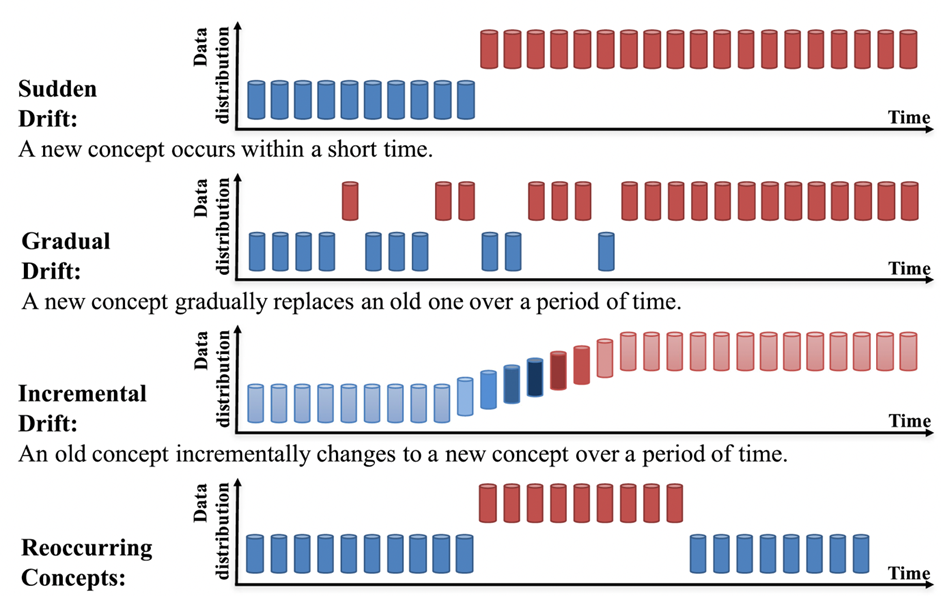
\includegraphics[width=0.8\textwidth]{2_Background/figures/concept_drift_types.png}
    \caption{Types of Concept Drift \cite{8496795}. \\ \textcolor{gray}{\fontsize{10}{0}\selectfont DOI: 10.1109/TKDE.2018.2876857}}
    \label{fig:concept-drift-types}
\end{figure}

